%
% STAT 100: Chance and Data Analysis - A Course Overview
% Section: Analysis of Single-Variable Data
%
% Author: Jeffrey Leung
%

\section{Analysis of Single-Variable Data}
	\label{sec:analysis-of-single-variable-data}
\subsection{Categorical Data}
	\label{subsec:analysis-of-single-variable-data:categorical-data}
\begin{easylist}	
	
	& Analysis using statistics, tables, and graphs:
		&& Identify all options for the categorical variable(s)
		&& Create a frequency table
			&&& Total the number of each option chosen
			&&& Use a two-way frequency table if necessary (see \emph{Two-way frequency table}, below)
		&& Calculate the percentage/proportion of each category
			&&& $\frac{frequency}{total\ sample\ size}$
		&& Use graphs to visually display the data
			&&& E.g. Pie chart, line chart, bar graph
		&& Summarize the data and draw conclusions
			&&& Several sentences
			&&& Describe which options are the most/least frequent
			&&& Do not simply reproduce the numbers
		
		\medskip
		&& E.g. A study was conducted on SFU students to determine their opinion (agree/neutral/disagree) on purchasing an iPad as a substitution of textbooks. See table~\ref{tab:ipad-textbook-replacement} for the results.

		\Deactivate
		\begin{table}[!htb]
			\centering
			\caption{Opinions of Students on iPads as Textbook Substitutions}
			\label{tab:ipad-textbook-replacement}
			\begin{tabular}{ r l }
				Student ID & Opinion \\
				\hline
				 1 & Disagree \\
				 2 & Disagree \\
				 3 & Neutral \\
				 4 & Neutral \\
				 5 & Neutral \\
				 6 & Agree \\
				 7 & Disagree \\
				 8 & Neutral \\
				 9 & Disagree \\
				10 & Disagree \\
				11 & Agree \\
				12 & Neutral \\
				13 & Agree \\
				14 & Disagree \\
				15 & Neutral \\
				16 & Neutral \\
				17 & Agree \\
				18 & Disagree \\
				19 & Agree \\
				20 & Neutral
			\end{tabular}
		\end{table}
		\Activate
		
		\smallskip
		Variable: Opinion on purchasing an iPad as a substitution for textbooks \\
		Categories: Agree, neutral, disagree
		
		\smallskip
		For the frequency and percentage table, see table~\ref{tab:ipad-textbook-replacement-freq-table}.
			
		\Deactivate
		\begin{table}[!htb]
			\centering
			\caption{Frequency and Percentage Table of Opinions of Students on iPads as Textbook Substitutions}
			\label{tab:ipad-textbook-replacement-freq-table}
			\begin{tabular}{ l r r }
				Opinion:	& Frequency:	& Percentage: \\
				\hline
				Agree		& 5 			& 25 \\
				Neutral		& 8 			& 40 \\
				Disagree	& 7 			& 35 \\
				\hline
				Total:		& 20			& 100
			\end{tabular}
		\end{table}
		\Activate
		
		\smallskip
		For the bar graph, see figure~\ref{fig:ipad-textbook-replacement-bar-graph}.
		
		\begin{figure}[!htb]
			\centering
			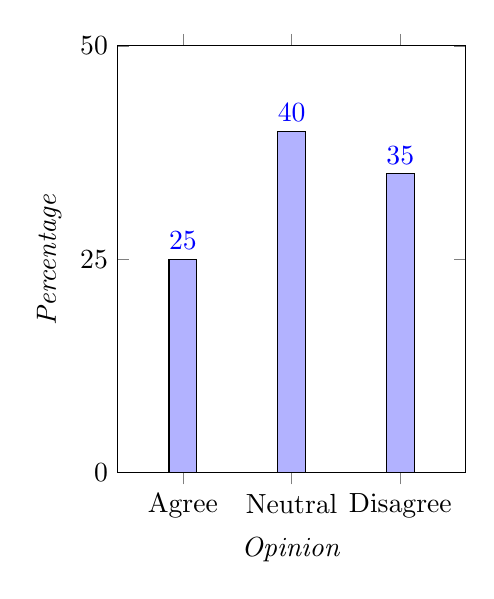
\begin{tikzpicture}
				\begin{axis}
					[
						enlarge x limits=0.3,
						%axis lines*=left, % Removes the top and right borders
						width=6cm,
						height=7cm,
						xtick=data,
						ybar,
						ymin=0,
						ymax=50,
						ytick={0, 25, 50},
						%bar width=\textwidth*.1,
						bar shift=0pt,
						symbolic x coords={Agree, Neutral, Disagree},
						nodes near coords,
						nodes near coords align = vertical,
						xlabel={\emph{Opinion}},
						ylabel={\emph{Percentage}}
					]
					\addplot+
						[
							draw=black
						]
						coordinates
						{
							(Agree, 25)
							(Neutral, 40)
							(Disagree, 35)
						};
				\end{axis}
			\end{tikzpicture}
			
			\caption{Bar Graph of Opinions of Students on iPads as Textbook Substitutions}
			\label{fig:ipad-textbook-replacement-bar-graph}
		\end{figure}
		
		\smallskip
		Conclusion: A large portion of students (40\%) stay neutral on purchasing an iPad as a substitution of textbooks. A small portion of students (25\%) agree on purchasing an iPad as a substitution of textbooks.
	
	& \emph{Two-way frequency table:} Table which allows the comparison of the frequency of two variables
		&& I.e. See table~\ref{tab:freq-table-example}
		
		\Deactivate
		\begin{table}[!htb]
			\centering
			\caption{Example of a two-way frequency table}
			\label{tab:freq-table-example}
			\begin{tabular}{ l l | r r | r }
				\multicolumn{2}{ c | }{} & \multicolumn{2}{ c | }{\emph{Var2}} & \\
				\multicolumn{2}{ c | }{} & Option1 & Option2 & \emph{Total:} \\
				\hline
				\multirow{2}{*}{\emph{Var1}}& Option1 & & & \\
				& Option2 & & & \\
				\hline
				\emph{Total:} & & & & 
			\end{tabular}
		\end{table}
		\Activate
		
		&& \emph{Side-by-side bar chart:} Display of multiple objects of study, each with multiple variable data (all objects sharing the same variables)
			&&& See figure~\ref{fig:side-by-side-bar-chart-example}

			\begin{figure}[!htb]
				\centering
				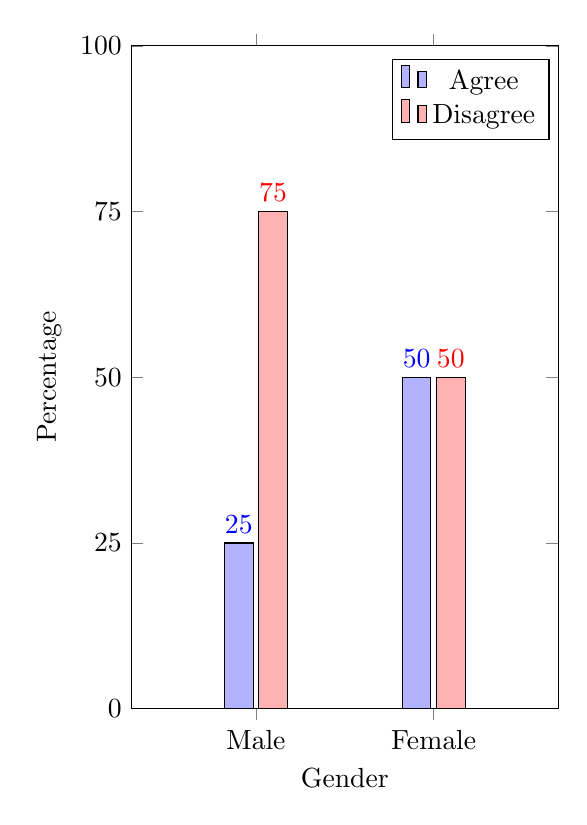
\begin{tikzpicture}
					\begin{axis}
						[
							enlarge x limits=0.7,
							%axis lines*=left, % Removes the top and right borders
							width=7cm,
							height=10cm,
							compat=newest,
							ybar,
							xtick=data,
							ymin=0,
							ymax=100,
							ytick={0, 25, 50, 75, 100},
							bar width=\textwidth*.03,
							symbolic x coords={Male, Female},
							nodes near coords,
							%nodes near coords align = vertical,z
							xlabel={Gender},
							ylabel={Percentage},
						]
						\addplot+
							[
								draw=black
							]
							coordinates
							{
								(Male, 25)
								(Female, 50)
							};
						\addplot+
							[
								draw=black
							]
							coordinates
							{
								(Male, 75)
								(Female, 50)
							};
						\legend{Agree, Disagree}
					\end{axis}
				\end{tikzpicture}
		
				\caption{Distribution of Agreement by Gender}
				\label{fig:side-by-side-bar-chart-example}
			\end{figure}
			
		&& Create $x$ bar charts to isolate analysis of each variable, where $x =$ number of variables per object of study
			&&& Compare the magnitude of the same choice in different sample groups
		
		&& Example: A study was conducted on the distribution of smokers by gender. The results were as follows: \\
		50\% of males smoked; 50\% of males did not smoke. \\
		20\% of females smoked; 80\% of females did not smoke.
		
		\medskip
		For the side-by-side bar graph, see figure~\ref{fig:distribution-of-smokers-by-gender}.
		
		\begin{figure}[!htb]
			\centering
			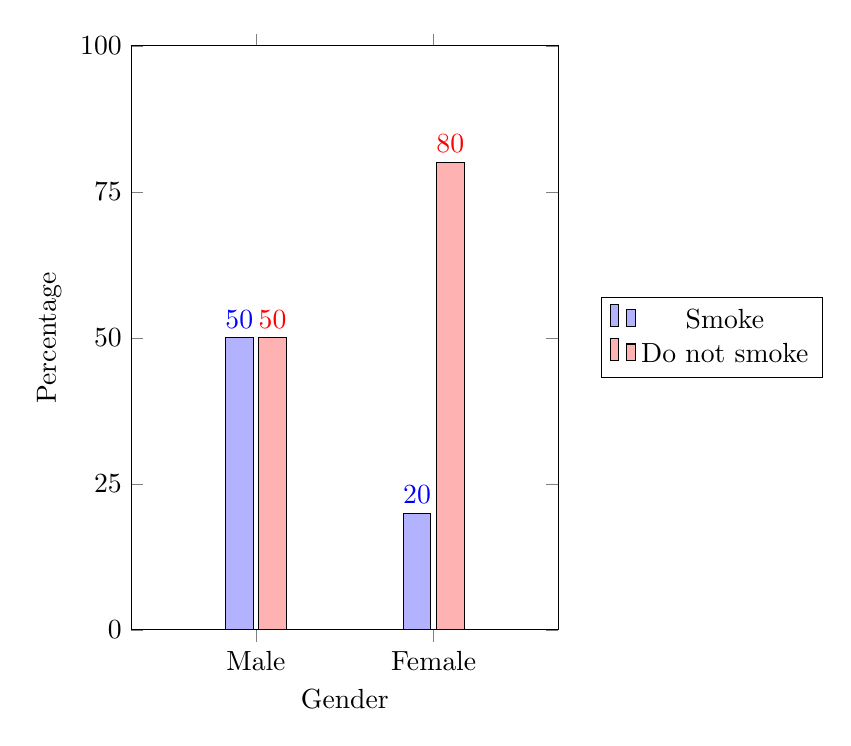
\begin{tikzpicture}
				\begin{axis}
					[
						% GRAPH:
						width=7cm,
						height=9cm,
						%axis lines*=left, % Removes the top and right borders
						% BARS:
						ybar, % Bar chart
						%bar width=\textwidth*.03,
						enlarge x limits=0.7, % Decreases distance between bars
						nodes near coords,
						nodes near coords align = vertical,
						% AXES:
						xtick=data,
						ytick={0, 25, 50, 75, 100},
						symbolic x coords={Male, Female},
						xlabel={Gender},
						ylabel={Percentage},
						ymin=0,
						ymax=100,
						%LEGEND:
						legend style={at={(1.1,0.5)},anchor=west},
					]
					\addplot+
						[
							draw=black
						]
						coordinates
						{
							(Male, 50)
							(Female, 20)
						};
					\addplot+
						[
							draw=black
						]
						coordinates
						{
							(Male, 50)
							(Female, 80)
						};
					\legend{Smoke, Do not smoke}
				\end{axis}
			\end{tikzpicture}
			
			\caption{Distribution of Smokers by Gender}
			\label{fig:distribution-of-smokers-by-gender}
		\end{figure}
		
		From figure~\ref{fig:distribution-of-smokers-by-gender:comparison-of-smokers}, the percentage of smokers is higher in the male group than the female group by 30\%.
		
		\begin{figure}[!htb]
			\centering
			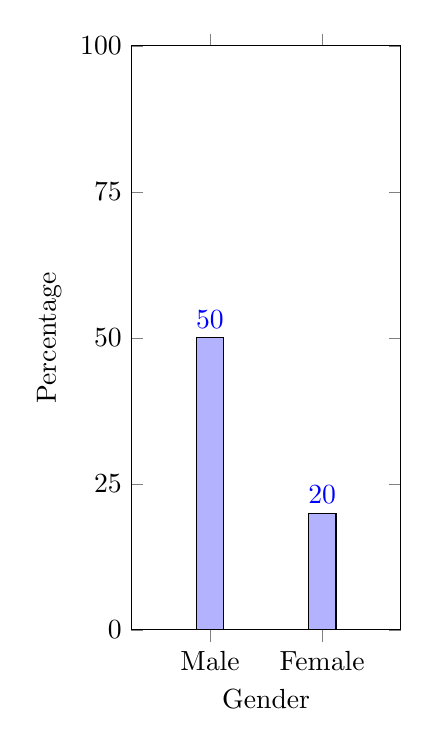
\begin{tikzpicture}
				\begin{axis}
					[
						% GRAPH:
						width=5cm,
						height=9cm,
						%axis lines*=left, % Removes the top and right borders
						% BARS:
						ybar, % Bar chart
						%bar width=\textwidth*.1,
						enlarge x limits=0.7, % Decreases distance between bars
						nodes near coords,
						nodes near coords align = vertical,
						% AXES:
						xtick=data,
						ytick={0, 25, 50, 75, 100},
						symbolic x coords={Male, Female},
						xlabel={Gender},
						ylabel={Percentage},
						ymin=0,
						ymax=100
					]
					\addplot+
						[
							draw=black
						]
						coordinates
						{
							(Male, 50)
							(Female, 20)
						};
				\end{axis}
			\end{tikzpicture}
			
			\caption{Comparison of Male and Female Smokers in a Distribution of Smokers by Gender}
			\label{fig:distribution-of-smokers-by-gender:comparison-of-smokers}
		\end{figure}
		
		From figure~\ref{fig:distribution-of-smokers-by-gender:comparison-of-nonsmokers}, the percentage of nonsmokers is higher in the female group than the male group by 30\%.
		
		\begin{figure}[!htb]
			\centering
			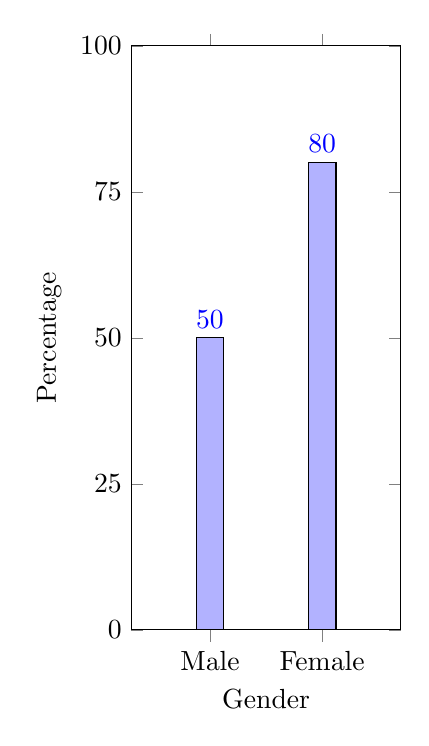
\begin{tikzpicture}
				\begin{axis}
					[
						% GRAPH:
						width=5cm,
						height=9cm,
						%axis lines*=left, % Removes the top and right borders
						% BARS:
						ybar, % Bar chart
						%bar width=\textwidth*.1,
						enlarge x limits=0.7, % Decreases distance between bars
						nodes near coords,
						nodes near coords align = vertical,
						% AXES:
						xtick=data,
						ytick={0, 25, 50, 75, 100},
						symbolic x coords={Male, Female},
						xlabel={Gender},
						ylabel={Percentage},
						ymin=0,
						ymax=100
					]
					\addplot+
						[
							draw=black
						]
						coordinates
						{
							(Male, 50)
							(Female, 80)
						};
				\end{axis}
			\end{tikzpicture}
			
			\caption{Comparison of Male and Female Non-Smokers in a Distribution of Smokers by Gender}
			\label{fig:distribution-of-smokers-by-gender:comparison-of-nonsmokers}
		\end{figure}

\end{easylist}
\subsection{Quantitative Data}
	\label{subsec:analysis-of-single-variable-data:quantitative-data}
\begin{easylist}	

	& Analysis using statistics, tables, and graphs:
		&& Divide the range of data into even classes
			&&& \emph{Class:} Range of values equal in length to all other classes, with no values between classes and no overlapping of classes
				&&&& I.e. Equal-length adjacent ranges of values
				&&&& E.g.  0-10, 10-20, 20-30
				&&&& All data must fall into exactly one class (i.e. there must be no value between classes, and the same value cannot be in multiple classes)
		&& Create a frequency table comparing the number of values in each class (see table~\ref{tab:freq-table-classes})
		
		\Deactivate
		\begin{table}[!htb]
			\centering
			\caption{Frequency Table with Classes}
			\label{tab:freq-table-classes}
			\begin{tabular}{ l r }
				Class Range: & Frequency: \\
				\hline
				$ 0 \leq value < 10$ & 5 \\
				$10 \leq value < 20$ & 4 \\
				$20 \leq value < 30$ & 3 \\
				$30 \leq value < 40$ & 2 \\
				$40 \leq value < 50$ & 1 \\
				\hline
				Total: & 15
			\end{tabular}
		\end{table}
		\Activate
		
		&& Create a histogram:
			&&& \emph{Histogram:} Visual display of classes of values against the frequency of data in each class (see figure~\ref{fig:histogram})
			
			\begin{figure}[!htb]
				\centering
				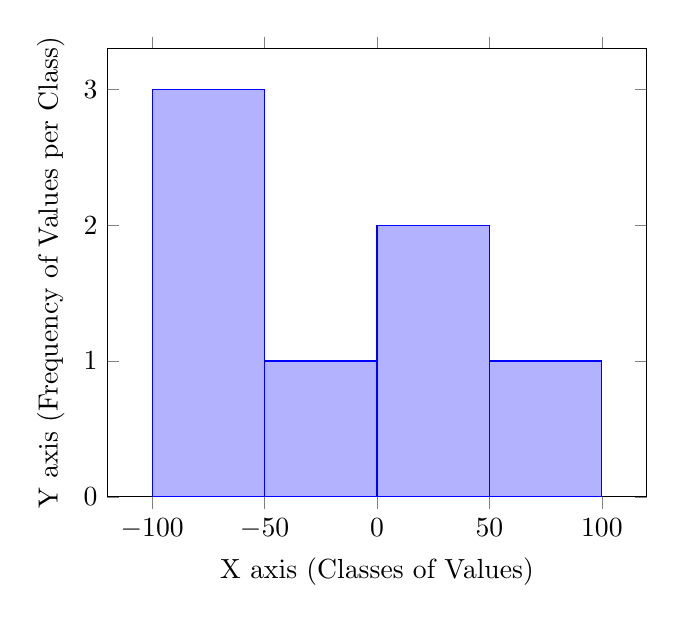
\begin{tikzpicture}[scale=1]
					\begin{axis}
					[
						ybar,
						ymin=0,
						xtick={-100, -50, 0, 50, 100},
						ytick={0, 1, 2, 3},
						xlabel=X axis (Classes of Values),
						ylabel=Y axis (Frequency of Values per Class)
					]
						\addplot +
						[
							hist=
							{
								bins=4,
								data min=-100,
								data max=100
							}
						] table [y index = 0]
						{
							-75
							-75
							-75
							-25
							25
							25
							75
						};
					\end{axis}
				\end{tikzpicture}
				
				\caption{Example of a Histogram}
				\label{fig:histogram}
			\end{figure}
			
			\medskip
			&& E.g. The annual salary (in thousands of dollars) of 10 random UBC graduates was found to be 16, 18, 25, 26, 28, 32, 38, 42, 55, and 80. \smallskip \\
			For the frequency table, see table~\ref{tab:ubc-graduates-salaries-freq-table}.

			\Deactivate
			\begin{table}[!htb]
				\centering
				\caption{Frequency Table of UBC Graduates' Salaries}
				\label{tab:ubc-graduates-salaries-freq-table}
				\begin{tabular}{ l r }
					Classes: & Frequency: \\
					\hline
					$15 \leq salary < 30$ & 5 \\
					$30 \leq salary < 45$ & 3 \\
					$45 \leq salary < 60$ & 1 \\
					$60 \leq salary < 75$ & 0 \\
					$75 \leq salary < 90$ & 1
				\end{tabular}
			\end{table}
			\Activate
			
			For the histogram, see figure~\ref{fig:ubc-graduates-salaries-histogram}.
			
			\begin{figure}[!htb]
				\centering
				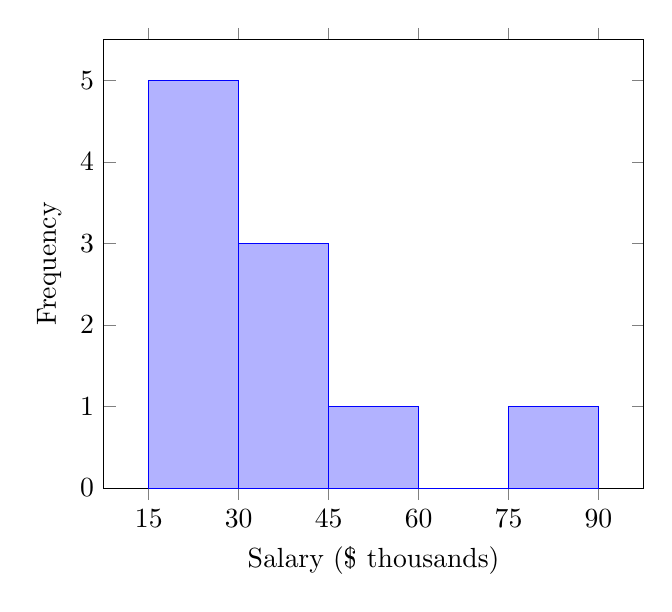
\begin{tikzpicture}[scale=1]
					\begin{axis} %TODO
					[
						ybar,
						ymin=0,
						xtick={15, 30, 45, 60, 75, 90},
						ytick={0, 1, 2, 3, 4, 5},
						xlabel=Salary (\$ thousands),
						ylabel=Frequency
					]
						\addplot +
						[
							hist=
							{
								bins=5,
								data min=15,
								data max=90
							}
						] table [y index = 0]
						{
							16
							18
							25
							26
							28
							32
							38
							42
							55
							80
						};
					\end{axis}
				\end{tikzpicture}
				
				\caption{Histogram of UBC Graduates' Salary}
				\label{fig:ubc-graduates-salaries-histogram}
			\end{figure}

\end{easylist}
\subsection{Statistics of Quantitative Data}
	\label{subsec:analysis-of-single-variable-data:statistics-of-quantitative-data}
\begin{easylist}

	& \emph{Minimum:} Least value in a set of data
	& \emph{Maximum:} Greatest value in a set of data
	& \emph{Range:} Area of values over which the data is spread; expressed in terms of the minimum and maximum
	& \emph{Median:} Number which 50\% of values are less than, and which 50\% of values are greater than
		&& Location in a table of ascending order: $\frac{n + 1}{2}$ where $n =$ the number of data points
			&&& If there are two middle numbers, the median is their average
		&& E.g. The median of values \{1, 3, 5, 7\} is located at $\frac{4+1}{2} = 2.5$. Therefore, the median is the average of the two middle values, which is $\frac{3+5}{2} = 4$.
		&& Example of interpretation: About 50\% of UBC graduates earn less than \$30,000 and the other 50\% of UBC graduates earn greater than \$30,000 per year.
	
	\medskip
	& \emph{Quartiles:} 3 points which divide the data into 4 groups, with the same amount of values in each group
		&& \emph{First quartile (Q1)}: Value which 25\% of the data is less than
			&&& I.e. Median of the lesser half of the data (the median itself is excluded)
		&& \emph{Third quartile (Q3)}: Value which 25\% of the data is greater than
			&&& I.e. Median of the greater half of the data (the median itself is excluded)
		&& Example of interpretation: \\
		About 25\% of UBC graduates earned less than \$25,000. \\
		About 25\% of UBC graduates earned more than \$42,000. \\
		Furthermore, about 50\% of UBC graduates earned between \$25,000 and \$42,000.
	
	\medskip
	& E.g. Given the 11 values \{1, 2, 3, 4, 5, 6, 7, 8, 9, 10, 11\}: (see table~\ref{tab:quantitative-data-statistics-example})
	
	\Deactivate
	\begin{table}[!htb]
		\centering
		\caption{11 Values as an Example of Quantitative Data Statistics}
		\label{tab:quantitative-data-statistics-example}
		\begin{tabular}{ l *{11}{ c } }
			Minimum = 1		& \begin{bfseries} 1 \end{bfseries} & 2 & 3 & 4 & 5 & 6 & 7 & 8 & 9 & 10 & 11 \\
			Maximum = 11	& 1 & 2 & 3 & 4 & 5 & 6 & 7 & 8 & 9 & 10 & \begin{bfseries} 11 \end{bfseries} \\
			Median = 6		& 1 & 2 & 3 & 4 & 5 & \begin{bfseries} 6 \end{bfseries} & 7 & 8 & 9 & 10 & 11 \\
			Q1 = 3			& 1 & 2 & \begin{bfseries} 3 \end{bfseries} & 4 & 5 & 6 & 7 & 8 & 9 & 10 & 11 \\
			Q3 = 9			& 1 & 2 & 3 & 4 & 5 & 6 & 7 & 8 & \begin{bfseries} 9 \end{bfseries} & 10 & 11
		\end{tabular}
	\end{table}
	\Activate
	
	& \emph{Five-number summary:} Description of data using 5 specific values (minimum, first quartile, median, third quartile, maximum)
		&& About 25\% of data falls between:
			&&& The minimum and Q1
			&&& Q1 and the median
			&&& The median and Q3
			&&& Q3 and the maximum
			
		&& \emph{Boxplot:} Visual display of the five-number summary (see figure~\ref{fig:boxplot-example})
			&&& Consists of a box bordered by Q1 and Q3, a vertical line in the box at the median, and two `tails' to the left and right of the box at the minimum and maximum
			
			\begin{figure}[!htb]
				\centering
				\begin{tikzpicture}
					\begin{axis}
					[
						xscale=1.7, % Size of figure
						yscale=.7,
						ytick=0,
						xlabel=X axis
					]
						\addplot+
						[
							boxplot prepared=
							{
								lower whisker=0,
								lower quartile=1,
								median=2,
								upper quartile=3,
								upper whisker=4
							},
						]
						coordinates {} ;
					\end{axis}
				\end{tikzpicture}
				
				\caption{Example of a Boxplot}
				\label{fig:boxplot-example}
			\end{figure}
			
			&&& \emph{Inter-quartile range:} Width of the box; difference between Q1 and Q3
			
	& \emph{Outlier:} Data point which falls outside the overall pattern
		&& E.g. 10 students write a final exam. 9 students received a mark below 60\%; 1 student received a mark of 100\%. The 1 student is an outlier.
		&& May occur due to chance or error
		&& Can be detected by:
			&&& A boxplot generated by statistical software (displayed as a plot outside the boxplot range)
			&&& Using the 1.5 IQR rule:
				&&&& \emph{Lower limit:} Q1 - 1.5 $\cdot$ IQR
				&&&& \emph{Upper limit:} Q3 + 1.5 $\cdot$ IQR
				&&&& Any point less than the lower limit or greater than the upper limit is an outlier
		&& E.g. The annual salary (in thousands) of 10 random UBC graduates was found to be 16, 18, 25, 26, 28, 32, 38, 42, 55, and 80. Detect any outliers. \smallskip \\
		Q1 = 25 \\
		Q3 = 38 \\
		IQR = Q3 - Q1 = 38 - 25 = 13 \\
		Lower limit = Q1 - 1.5 $\cdot$ IQR = 25 - 1.5 $\cdot$ 13 = 5.5 \\
		Upper limit = Q3 + 1.5 $\cdot$ IQR = 38 + 1.5 $\cdot$ 13 = 57.5 \smallskip \\
		The outlier is 80, because it is the only data point less than the lower limit or greater than the upper limit.
				
\end{easylist}
\subsection{Shape, Center, and Spread of a Distribution}
	\label{subsec:analysis-of-single-variable-data:shape-center-spread-of-a-distribution}
\begin{easylist}

	& \emph{Shape (distribution):} Skew of data points or lack thereof
		&& Calculated through the distances between Q1 and the median, and the median and Q3
		
		&& \emph{Skewed to the left:} Most data points are mainly on the right side of the distribution
			&&& Tail of data on the left; bulge of data on the right
			&&& $median - Q1 > Q3 - median$
			&&& E.g. See figure~\ref{fig:distribution-skewed-to-the-left}
			
			\begin{figure}[!htb]
				\centering
				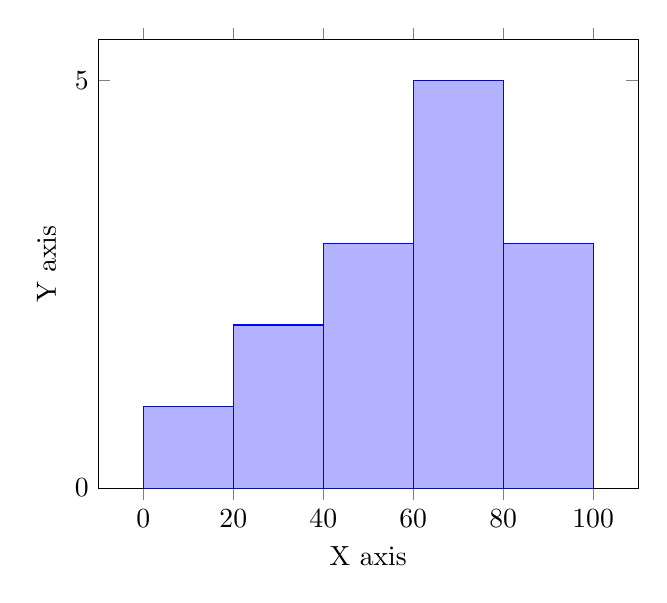
\begin{tikzpicture}
					\begin{axis}
					[
						ybar,
						ymin=0,
						xtick={0, 20, 40, 60, 80, 100},
						ytick={0, 5},
						xlabel=X axis,
						ylabel=Y axis
					]
						\addplot +
						[
							hist=
							{
								bins=5,
								data min=0,
								data max=100
							}
						] table [y index = 0]
						{
							10
							30
							30
							50
							50
							50
							70
							70
							70
							70
							70
							90
							90
							90
						};
					\end{axis}
				\end{tikzpicture}
				
				\caption{Example of a Distribution Skewed to the Left}
				\label{fig:distribution-skewed-to-the-left}
			\end{figure}
			
		&& \emph{Normal distribution:} Most data points are mainly in the centre of the distribution
			&&& Tails of data on the right and left; bulge of data in the centre
			&&& $median - Q1 \approx Q3 - median$
			&&& See subsection~\ref{subsec:analysis-of-single-variable-data:normal-distribution}
			&&& E.g. See figure~\ref{fig:distribution-normal}
			
			\begin{figure}[!htb]
				\centering
				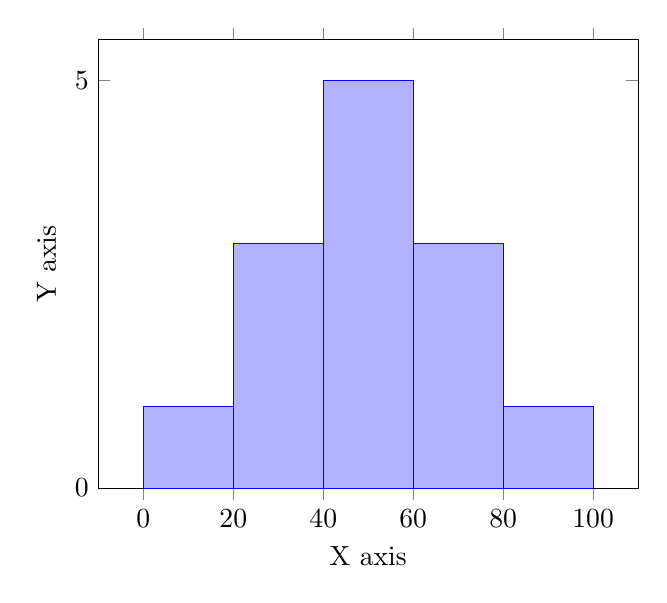
\begin{tikzpicture}[scale=1]
					\begin{axis}
					[
						ybar,
						ymin=0,
						xtick={0, 20, 40, 60, 80, 100},
						ytick={0, 5},
						xlabel=X axis,
						ylabel=Y axis
					]
						\addplot +
						[
							hist=
							{
								bins=5,
								data min=0,
								data max=100
							}
						] table [y index = 0]
						{
							10
							30
							30
							30
							50
							50
							50
							50
							50
							70
							70
							70
							90
						};
					\end{axis}
				\end{tikzpicture}
				
				\caption{Example of a Normal Distribution Skewed to the Right}
				\label{fig:distribution-normal}
			\end{figure}
			
		&& \emph{Skewed to the right:} Most data points are mainly on the left side of the distribution
			&&& Tail of data on the right; bulge of data on the left
			&&& $median - Q1 < Q3 - median$
			&&& E.g. See figure~\ref{fig:distribution-skewed-to-the-right}
			
			\begin{figure}[!htb]
				\centering
				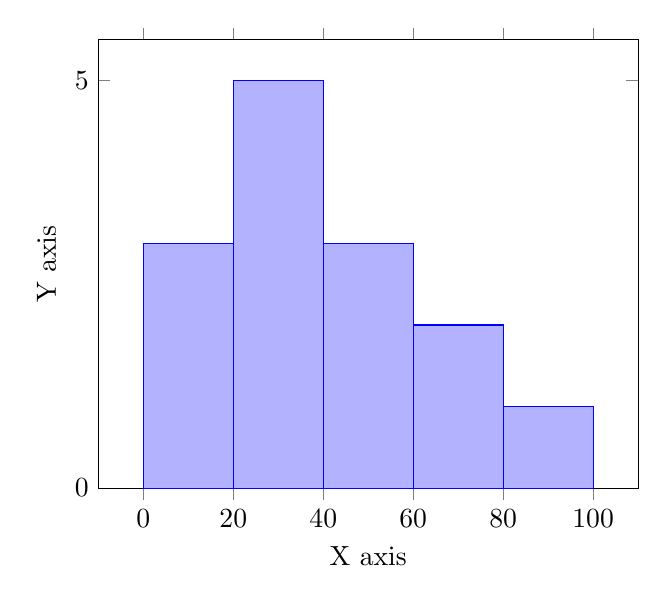
\begin{tikzpicture}[scale=1]
					\begin{axis}
					[
						ybar,
						ymin=0,
						xtick={0, 20, 40, 60, 80, 100},
						ytick={0, 5},
						xlabel=X axis,
						ylabel=Y axis
					]
						\addplot +
						[
							hist=
							{
								bins=5,
								data min=0,
								data max=100
							}
						] table [y index = 0]
						{
							10
							10
							10
							30
							30
							30
							30
							30
							50
							50
							50
							70
							70
							90
						};
					\end{axis}
				\end{tikzpicture}
				
				\caption{Example of a Distribution Skewed to the Right}
				\label{fig:distribution-skewed-to-the-right}
			\end{figure}
			
		&& Correspond directly to the boxplot
		&& Extreme values affect the mean more than the median:
			&&& Skewed to the left: Mean is less than the median
			&&& Normal distribution: Mean is roughly equal to the median
			&&& Skewed to the right: Mean is greater than the median
			
		\medskip
		&& E.g. The annual salary (in thousands) of 10 random UBC graduates was recorded and analyzed. See table~\ref{tab:ubc-graduates-five-number-summary} for the five-number summary.
		
		\Deactivate
		\begin{table}[!htb]
			\centering
			\caption{Five-Number Summary of UBC Graduates' Annual Salaries}
			\label{tab:ubc-graduates-five-number-summary}
			\begin{tabular}{ l r }
				Minimum & 16 \\
				Q1 & 25 \\
				Median & 30 \\
				Q3 & 42 \\
				Maximum & 80
			\end{tabular}
		\end{table}
		\Activate
		
		Median - Q1 = 30 - 25 = 5 \\
		Q3 - median = 42 - 30 = 12 \\
		Since the distance between the median and Q3 is greater than the distance between Q1 and the median, the distribution is skewed to the right.
		
		%TODO Weeks 1/2, Document 03, Page 3
				
	& \emph{Center:} Median of a distribution
		&& Used for general comparisons of magnitude
		
	& \emph{Spread/variability:} How data points are distributed across the range
		&& Often measured by IQR (see \emph{inter-quartile range}, subsection~\ref{subsec:analysis-of-single-variable-data:categorical-data})
			&&& The greater the IQR, the greater the spread
		&& Not often measured by range because it is affected greatly by outliers
			&&& Only used when a conclusion cannot be derived using the IQR

	& UBC study %TODO
	
	& E.g. Boxplot and summary statistics \smallskip \\ %TODO
	The shape is skewed to the right. \\
	The median exam score is 60\%. Therefore, about 50\% of students scored less than 60\%, while the other 50\% of students scored higher than 60\%. \\
	The spread: Ranges from 55\% min to 92\% max. The middle 50\% of exam scores are between 58\% at Q1 and 66.5\% at Q3. \\
	There are 2 outliers; therefore, 2 students received abnormally high exam scores.

	& \emph{Mean/Average:} Sum of a set of values divided by the number of values
		&& Denoted by an overline ($\overline{x}$)

	& \emph{Standard deviation:} 
		&& Denoted by $\sigma$
		&& Formula:
		\begin{displaymath}
		\sigma =
		\sqrt
		{
			\frac
			{
				\sum \limits_{i=0}^n (x_{i} - \overline{x})^2
			}
			{
				n - 1
			}
		}
		\end{displaymath}
		\Deactivate
		\begin{center}
			\begin{tabular}{ l r @{ = } l }
				where: & $x$ & variable data \\
				& $\overline{x}$ & mean of the variable data \\
				& $n$ & total number of sample data points
			\end{tabular}
		\end{center}
		\Activate
		
	& %TODO example, other
	
\end{easylist}
\subsection{Normal Distributions}
	\label{subsec:analysis-of-single-variable-data:normal-distribution}
\begin{easylist}

	& Use a mean and standard deviation to analyze a normal distribution
		
	& %TODO
	
	& \emph{Standard (z-) score:} 
		&& Formula: $z = \frac{x - mean}{s}$ %TODO LEGEND - s = standard deviation
			&&& $x = mean + z \cdot s$
		&& Shade the region of interest and use the standard normal table to find the corresponding percentage
			&&& Only calculate the z-score up to one significant digit
			&&& Standard normal table gives area to the left of the z-score; if the z-score is positive ( is greater than the mean), subtract it from 100\%
		&& Example: %TODO
	
\end{easylist}
\clearpage